%%%%%%%%%%%%%%%%%%%%%%%%%%%%%%%%%%%%%%%%%
% Beamer Presentation
% LaTeX Template
% Version 1.0 (10/11/12)
%
% This template has been downloaded from:
% http://www.LaTeXTemplates.com
%
% License:
% CC BY-NC-SA 3.0 (http://creativecommons.org/licenses/by-nc-sa/3.0/)
%
%%%%%%%%%%%%%%%%%%%%%%%%%%%%%%%%%%%%%%%%%

%----------------------------------------------------------------------------------------
%	PACKAGES AND THEMES
%----------------------------------------------------------------------------------------

\documentclass{beamer}

\mode<presentation> {

% The Beamer class comes with a number of default slide themes
% which change the colors and layouts of slides. Below this is a list
% of all the themes, uncomment each in turn to see what they look like.

%\usetheme{default}
%\usetheme{AnnArbor}
%\usetheme{Antibes}
%\usetheme{Bergen}
%\usetheme{Berkeley}
%\usetheme{Berlin}
%\usetheme{Boadilla}
%\usetheme{CambridgeUS}
%\usetheme{Copenhagen}
%\usetheme{Darmstadt}
%\usetheme{Dresden}
%\usetheme{Frankfurt}
%\usetheme{Goettingen}
%\usetheme{Hannover}
%\usetheme{Ilmenau}
%\usetheme{JuanLesPins}
%\usetheme{Luebeck}
\usetheme{Madrid}
%\usetheme{Malmoe}
%\usetheme{Marburg}
%\usetheme{Montpellier}
%\usetheme{PaloAlto}
%\usetheme{Pittsburgh}
%\usetheme{Rochester}
%\usetheme{Singapore}
%\usetheme{Szeged}
%\usetheme{Warsaw}
\usepackage{graphicx}
\usepackage{subfigure}
\usepackage{color}
\definecolor{answer}{RGB}{151,255,255}
% As well as themes, the Beamer class has a number of color themes
% for any slide theme. Uncomment each of these in turn to see how it
% changes the colors of your current slide theme.

%\usecolortheme{albatross}
%\usecolortheme{beaver}
%\usecolortheme{beetle}
%\usecolortheme{crane}
%\usecolortheme{dolphin}
%\usecolortheme{dove}
%\usecolortheme{fly}
%\usecolortheme{lily}
%\usecolortheme{orchid}
%\usecolortheme{rose}
%\usecolortheme{seagull}
%\usecolortheme{seahorse}
%\usecolortheme{whale}
%\usecolortheme{wolverine}

%\setbeamertemplate{footline} % To remove the footer line in all slides uncomment this line
%\setbeamertemplate{footline}[page number] % To replace the footer line in all slides with a simple slide count uncomment this line

%\setbeamertemplate{navigation symbols}{} % To remove the navigation symbols from the bottom of all slides uncomment this line
}

\usepackage{graphicx} % Allows including images
\usepackage{booktabs} % Allows the use of \toprule, \midrule and \bottomrule in tables

%----------------------------------------------------------------------------------------
%	TITLE PAGE
%----------------------------------------------------------------------------------------

\title[Midterm RC]{VY100 Midterm Exam Recitation} % The short title appears at the bottom of every slide, the full title is only on the title page

\author{Ma Ziqiao} % Your name
\institute[UM-SJTU JI] % Your institution as it will appear on the bottom of every slide, may be shorthand to save space
{
UM-SJTU Joint Institute \\ % Your institution for the title page
\medskip
\textit{martin\underline{ }maziqiao@sjtu.edu.com} % Your email address
}
\date{\today} % Date, can be changed to a custom date

\begin{document}

\begin{frame}
\titlepage % Print the title page as the first slide
\end{frame}

\begin{frame}
\frametitle{Overview} % Table of contents slide, comment this block out to remove it
\tableofcontents % Throughout your presentation, if you choose to use \section{} and \subsection{} commands, these will automatically be printed on this slide as an overview of your presentation
\end{frame}

%----------------------------------------------------------------------------------------
%	PRESENTATION SLIDES
%----------------------------------------------------------------------------------------

%------------------------------------------------
\section{Arguing through Art} 
\subsection{Painting} 
%------------------------------------------------
\begin{frame}
\frametitle{Paintings}
\begin{columns}[c] % The "c" option specifies centered vertical alignment while the "t" option is used for top vertical alignment

\column{.3\textwidth} % Left column and width
\textbf{Guidelines}
\begin{itemize}
\item Line
\item Color
\item Shape $\&$ Form
\item Texture
\item Perspective
\end{itemize}

\column{.5\textwidth} % Right column and width
\begin{itemize}
\item Composition $\&$ Balance
\item Proportion
\item Variety
\item Movement
\item Space
\end{itemize}

\end{columns}
\end{frame}

%----------------------------------------------
\begin{frame}
\frametitle{Paintings}
\begin{block}{Line}
Defined by a point moving in space. 
\begin{itemize}
\item Line may be \textbf{two-or three-dimensional}(Curves included), descriptive, implied, or abstract. 
\item Different lines give different feelings.
\end{itemize}

\end{block}

\begin{block}{Color}
Made up of three properties: \textbf{hue, value, and intensity}.
\begin{itemize}
\item Hue: Name of color .
\item Value: Hue's lightness and darkness (a color’s value changes when white or black is added) 
\item Intensity: Quality of brightness and purity.
	\begin{itemize}
	\item High intensity: color is strong and bright.
	\item Low intensity: color is faint and dull.
	\end{itemize}
\end{itemize}
\end{block}
\end{frame}
%------------------------------------------------
\begin{frame}
\frametitle{Paintings}
\begin{block}{Shape and Form}
\begin{itemize}
\item Shape is an element of art that is \textbf{two-dimensional}, flat, or limited to height and width.
\item Form is an element of art that is \textbf{three-dimensional} and encloses volume; includes height, width and depth (as in a cube, a sphere, a pyramid, or a cylinder). Form may also be free flowing. 
\end{itemize}
\end{block}

\begin{block}{Texture}
Refers to the way things feel, or look as if they might feel if touched.
\end{block}

\begin{block}{Perspective}
The point of view of the painting. It describes where the painter standing in relation to the subject.
\end{block}
\end{frame}
%------------------------------------------------
\begin{frame}
\frametitle{Paintings}
\begin{block}{Composition and Balance}
A way of combining elements to add a feeling of equilibrium or stability to a work of art. Major types are \textbf{symmetrical} and \textbf{asymmetrical}.
\begin{itemize}
\item Asymmetrical composition aims at attracting viewers' attention to (away from) certain parts of the painting.
\end{itemize}
\end{block}

\begin{block}{Proportion}
The relationship of certain elements to the whole and to each other.
\begin{itemize}
\item Proportion involves comparison. You can't simply say one element is big. Make comparison with the whole painting or other elements.
\end{itemize}
\end{block}
\end{frame}
%------------------------------------------------
\begin{frame}
\frametitle{Paintings}
\begin{block}{Variety}
\begin{itemize}
\item A principle of design concerned with diversity or contrast. 
\item Variety is achieved by using different shapes, sizes, and/or colors in a work of art. Emphasis can be created by creating contrasts.
\end{itemize}
\end{block}

\begin{block}{Movement}
A principle of design used to create the look and feeling of action and to guide the viewers' eyes throughout the work of art. The painting is still. The scene is not.
\end{block}

\begin{block}{Space}
An element of art by which positive and negative areas are defined or a sense of depth achieved in a work of art.
\end{block}
\end{frame}
%------------------------------------------------
\begin{frame}
\frametitle{Paintings}
List the techniques used in the paintings and explain why.
\begin{figure}[!htbp] 
\centering 
\subfigure[A Kidnapped Mum]{
	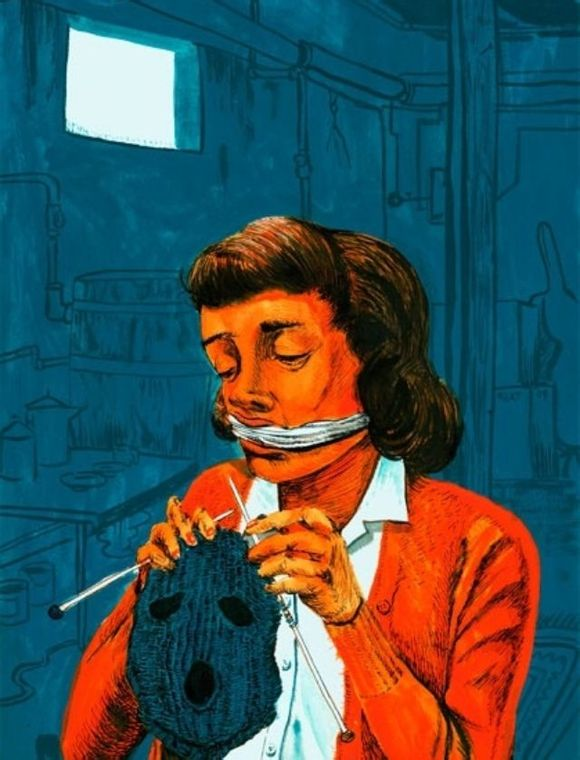
\includegraphics[width=0.4\linewidth]{painting1.jpg}  
	\label{fig-1} 
}
\subfigure[Bedtime]{
	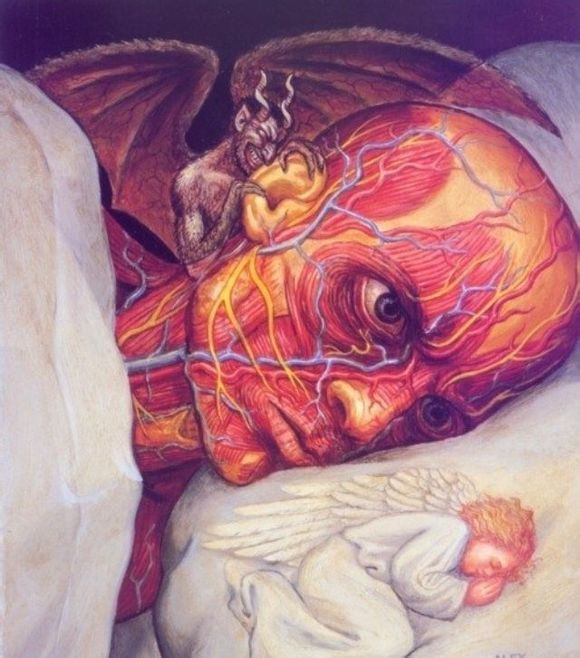
\includegraphics[width=0.4\linewidth]{painting2.jpg} 
	\label{fig-2} 
}
\caption{Exercise} 
\end{figure}
\end{frame}
%------------------------------------------------
\subsection{Poetry}
\begin{frame}
\frametitle{Poems}
\begin{columns}[c] % The "c" option specifies centered vertical alignment while the "t" option is used for top vertical alignment

\column{.45\textwidth} % Left column and width
\begin{enumerate}
\item \textbf{Stanza}

A paragraph.
\item \textbf{Line}

The basic measurement.
\item \textbf{Sentence}

Grammatically full sentence.
\end{enumerate}

\column{.5\textwidth} % Right column and width
\textbf{Example}\\
Twinkle, twinkle, little star,\\
How I wonder what you are!\\
Up above the world so high,\\
Like a diamond in the sky.\\
\vspace{2ex}
When this blazing sun is gone,\\
When he nothing shines upon,\\
Then you show your little light,\\
Twinkle, twinkle, through the night.
\end{columns}
\end{frame}
%------------------------------------------------
\begin{frame}
\frametitle{Poems}
\begin{columns}[c] % The "c" option specifies centered vertical alignment while the "t" option is used for top vertical alignment

\column{.4\textwidth} % Left column and width
\begin{itemize}
\item \textbf{Couplet}

Two lines that are connected by rhyme.
\item \textbf{Meter}

How the poem sounds. (Rhythm)
\end{itemize}

\column{.6\textwidth} % Right column and width
\textbf{Example}\\
Gather ye rosebuds while ye may,\qquad\qquad A\\
Old Time is still a-flying: \qquad\qquad\qquad\quad B\\
And this same flower that smiles to-day,\quad A\\
To-morrow will be dying. \qquad\qquad\qquad\quad B
\end{columns}
\vspace{4ex}
\begin{block}{Free Verse and Prose}
\begin{itemize}
\item \textbf{Free verse poetry} has no rhyme or meter to it. 
\item \textbf{Prose} is normal writing. It's essays and short stories. It's most writing that isn't poetry.
\end{itemize}
\end{block}

\end{frame}
%------------------------------------------------
\begin{frame}
\frametitle{Poems}
\begin{block}{Speaker and Audience}
\begin{itemize}
\item All poems have a speaker.
\item Poems may have a specific audience.
\item $\Box$ Speaker = Poet.
\item $\Box$ Speaker is not real, he is fictitious.
\end{itemize}
\end{block}

\begin{block}{Imagination}
Imagery is when a specific image is being formed by the author. When you can see something in a poem.
\end{block}

\begin{block}{Abstract and Concrete}
\begin{itemize}
\item \textbf{Abstract}: "The $price$ of $liberty$ is eternal $vigilance$."
\item \textbf{Concrete}: "The $moon$ stood in the $sky$, a lone $boy$ waiting for his love."
\end{itemize}
\end{block}
\end{frame}
%------------------------------------------------
\begin{frame}
\frametitle{Poems}
\begin{block}{Smile and Metaphor}
Simile and metaphor are when two things are being compared.
\begin{itemize}
\item \textbf{Simile} uses $like$ and $as$ to compare. 
\item \textbf{Metaphor} says it simply is something else. 
\end{itemize}
\end{block}

\begin{block}{Tone}
Tone is how the poet sounds.
\begin{itemize}
\item Close/Far
\item Formal/Informal
\item Education Background 
\item Age and Sex
\end{itemize}
\end{block}
\end{frame}
%------------------------------------------------
\begin{frame}
\frametitle{Poems}
\begin{block}{Hyperbole}
Hyperbole is any exaggeration made for effect.
\end{block}

\begin{block}{Irony}
\begin{itemize}
\item \textbf{Verbal irony} is when the words themselves form a bit of a joke. 
\item \textbf{Dramatic irony} is someone says or does something that has two meanings. Only one meaning being known to the character. 
\item \textbf{Cosmic irony} refer to strange occurrences in daily life.
\end{itemize}
\end{block}
\end{frame}
%------------------------------------------------
\begin{frame}
\frametitle{Poems}
\textbf{Exercises}
\begin{block}{Smile and Metaphor}
\begin{itemize}
\item "All the world's a stage, And all the men and women merely players."
\item "O My Luve's like a red, red rose."
\end{itemize}
\end{block}

\begin{block}{Hyperbole and Irony}
\begin{itemize}
\item A character named Veritas always telling lies. 

(Veritas means truth in Latin)
\item "The bag weighed a ton."
\end{itemize}
\end{block}
\end{frame}
\subsection{Discourse Analysis}
%------------------------------------------------
\begin{frame}
\frametitle{Discourse Analysis}
\textbf{Basic Concepts}
\begin{block}{Discourse}
Connected text (spoken, written, signed) above the level of sentence.
\end{block}

\begin{block}{Utterance}
The realization of a given unit of speech on a specific occasion in a specific context.

\textbf{Utterance is the basic unit of spoken discourse.}
\end{block}

\begin{block}{Speech Act Theory}
Language performs actions.
\end{block}
\end{frame}
%------------------------------------------------
\begin{frame}
\frametitle{Discourse Analysis}
\begin{block}{Components of Speech Acts}
\begin{itemize}
\item Locutionary act: Referential meaning.
\item Illocutionary act: Intended meaning.
\item Prelocutionary act: Understood meaning.
\item Illocutionary force: Illocutionary Act and Prelocutionary Act.
\end{itemize}
\end{block}

\begin{block}{Direct/Indirect Speech Acts}
\begin{itemize}
\item Direct speach act: Locutionary act $=$ Illocutionary act.
\item Indirect speach act: Locutionary act $\neq$ Illocutionary act.
\end{itemize}
\end{block}
\end{frame}
%------------------------------------------------
\begin{frame}
\frametitle{Discourse Analysis}
\textbf{Types of Illocutionary Acts}
\begin{figure}[!htbp]
\center
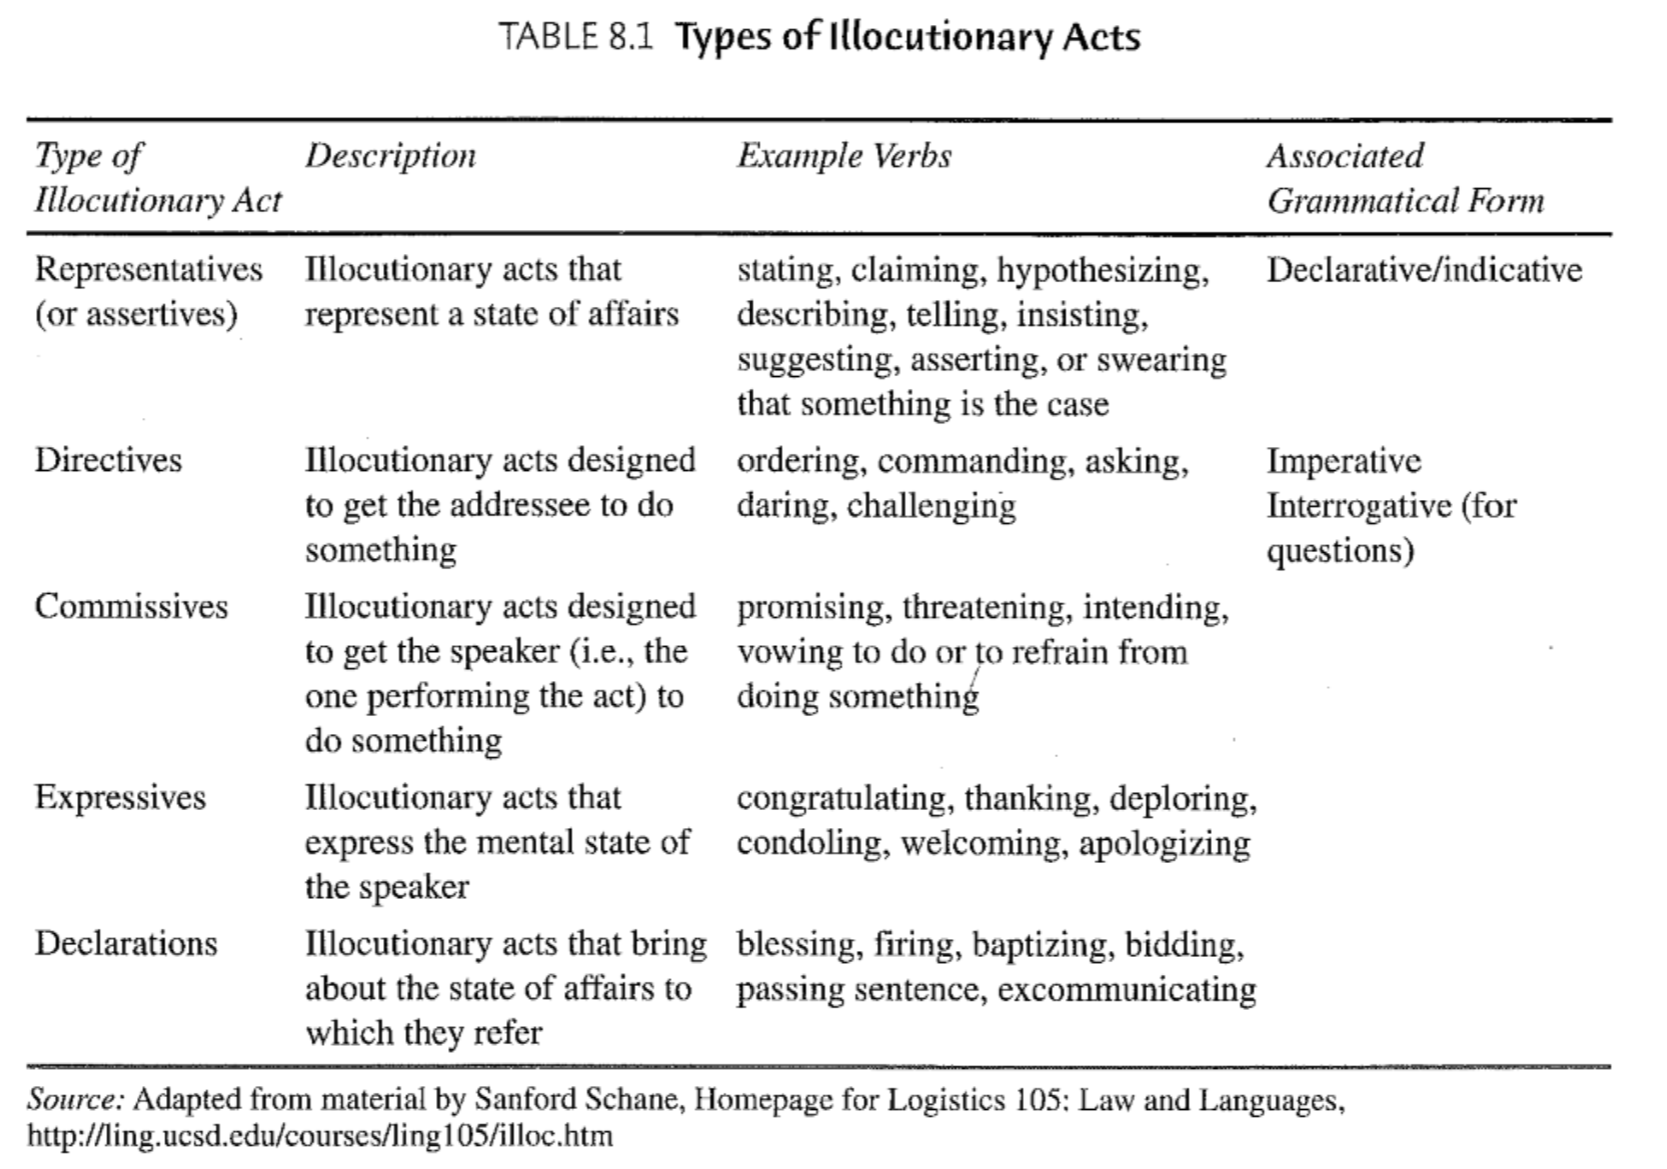
\includegraphics[width=10cm]{illo.png}
\end{figure}
\end{frame}
%------------------------------------------------
\begin{frame}
\frametitle{Discourse Analysis}
\begin{block}{Performative Speech Acts}
Utterances that explicitly state the action speaker performs.
\begin{itemize}
\item Employ 1$^{\text{st}}$-person subjects (I, we).
\item Employ present-tense verbs.
\end{itemize}
\end{block}

\begin{block}{The Cooperative Principle}
Make conversational contribution as is required, at the satge at which it occurs, by the accepted purpose or direction of talk exchange in which you are engaged.
\end{block}
\end{frame}
%------------------------------------------------
\begin{frame}
\frametitle{Discourse Analysis}
\begin{block}{Conversational Maxims}
\begin{itemize}
\item Maxims of Quantity.
	\begin{enumerate}
	\item As informative as is required.
	\item No more informative that required.
	\end{enumerate}
\item Maxims of Quality.
	\begin{enumerate}
	\item Don't say what you believe to be false.
	\item Don't say what you lack adequate evidence.
	\end{enumerate}
\item Maxims of Relation.
	\begin{enumerate}
	\item Don't say what is irrelevant to the topic.
	\end{enumerate}
\item Maxims of Manner.
	\begin{enumerate}
	\item Avoid obscurity.
	\item Avoid Ambiguity.
	\item Be brief.
	\item Be orderly.
	\end{enumerate}
\end{itemize}
\end{block}
\end{frame}
%------------------------------------------------
\begin{frame}
\frametitle{Discourse Analysis}
\begin{block}{Rules of Politeness}
\begin{itemize}
\item \textbf{Formality/Distance}: No impose, be aloof.
\item \textbf{Hesitancy/Deference}:Give others options about how to respond.
\item \textbf{Equality/Camaraderie}: Act like equal.
\end{itemize}
\end{block}

\begin{block}{Faces}
\begin{itemize}
\item \textbf{Positive faces}: The desire to be approved/liked.
\item \textbf{Negative faces}: The desire to be unimpeded.
\end{itemize}
\end{block}

\begin{block}{Politeness}
\begin{itemize}
\item \textbf{Positive politeness}: Enhance positive faces.
\item \textbf{Negative politeness}: Enhance negative faces.
\end{itemize}
\end{block}
\end{frame}
%------------------------------------------------
\begin{frame}
\frametitle{Discourse Analysis}
\textbf{Examples of Politeness}
\begin{figure}[!htbp]
\center
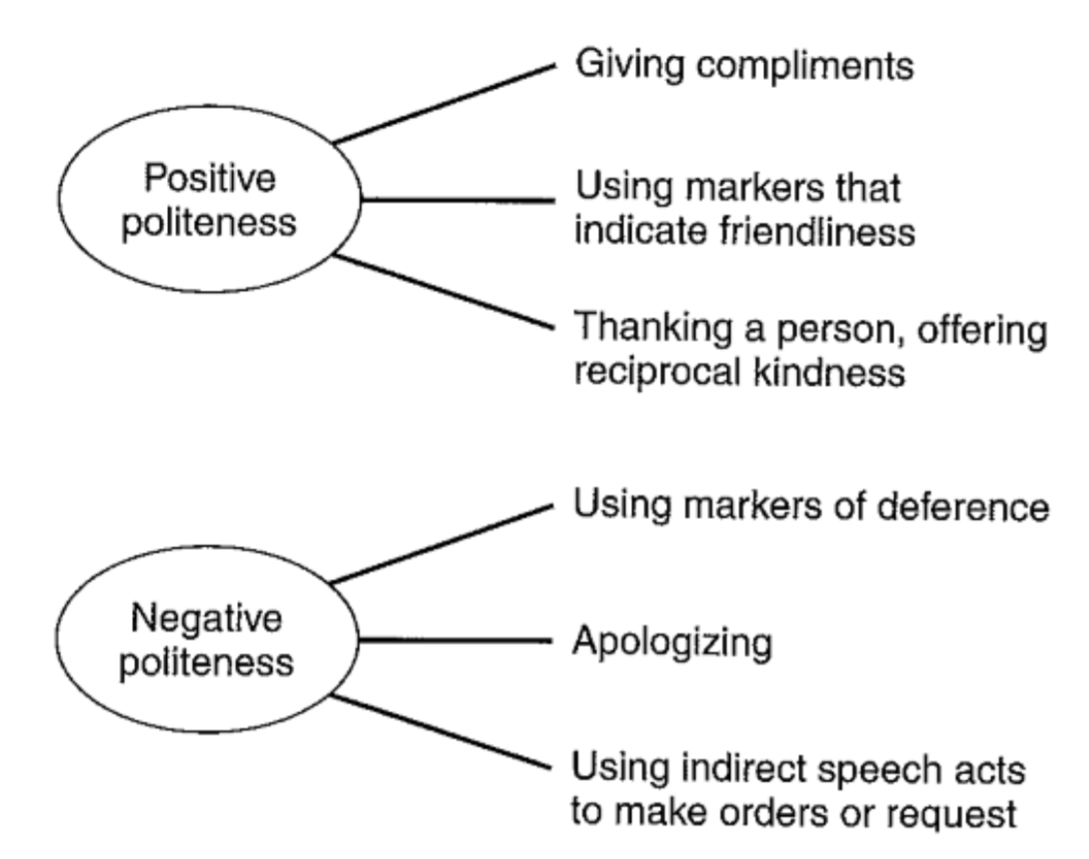
\includegraphics[width=8cm]{polite.png}
\end{figure}
\end{frame}
%------------------------------------------------
\begin{frame}
\frametitle{Discourse Analysis}
\begin{block}{Discourse Makes}
Semmingly meaningless elements in spoken language.
\begin{itemize}
\item \textbf{Adverbs}: so, however, then...etc
\item \textbf{Interjections}: oh, geez...etc
\item \textbf{verbs}: say, look...etc
\item \textbf{conjunctions}: and, but...etc
\item \textbf{Lexicalized clauses}: you know, I mean...etc
\end{itemize}
\end{block}
You should be able to list some functions of common discourse makers. They can be found on p.261.
\end{frame}
%------------------------------------------------
\begin{frame}
\frametitle{Discourse Analysis}
\begin{block}{Indications of Turn-taking}
\begin{columns}[c] 
\column{.3\textwidth}
\begin{itemize}
\item Silence
\item Questions
\item Gestures
\end{itemize}
\column{.3\textwidth} 
\begin{itemize}
\item Eye contact
\item Intonation
\end{itemize}
\end{columns}
\end{block}

\begin{block}{Violations of Turn-taking}
\begin{itemize}
\item Overlap
\item Interruption
\item Back-channelling
\end{itemize}
\end{block}

\begin{block}{Maintenance and Repair}
\begin{itemize}
\item All participants have to work to maintain a conversation: question-answer, invitation-respond.
\item Repair can be \textbf{self-initiated} and \textbf{other-initiated}.
\end{itemize}
\end{block}
\end{frame}
%------------------------------------------------
\begin{frame}
\frametitle{Discourse Analysis}
\textbf{Exercises}
\begin{block}{Types of Illocutionary Acts}
\begin{itemize}
\item "Give me full marks or I will kill you."
\item "I swear I handed in my essay yesterday!"
\item "Thanks a billion for your help."
\end{itemize}
\end{block}

\begin{block}{Violation of Conversational Maxims}
\begin{itemize}
\item "He's got full marks, I guess."
\item - "What did Ryan teach today?"\\
\quad "Discourse analysis. After that I went to Horst's class."
\end{itemize}
\end{block}

\begin{block}{Means of Violation of Turn-taking}
\begin{itemize}
\item[-] "Martin is super cool, you know?"
\item[-] "Yeah, I know! He is the best TA ever."
\end{itemize}
\end{block}

\end{frame}
%------------------------------------------------
\section{Crafting Essay}
\subsection{Grammar Mistakes}
%------------------------------------------------
\begin{frame}
\frametitle{Grammar Mistakes}
\begin{columns}[c] % The "c" option specifies centered vertical alignment while the "t" option is used for top vertical alignment

\column{.5\textwidth} % Left column and width
\textbf{Guidelines}
\begin{itemize}
\item Wrong word
\item Missing comma after an	introductory element
\item Incomplete or	missing documentation
\item Vague pronoun reference
\item Spelling (including homonyms)
\item Mechanical error with a quotation
\item Unnecessary comma
\item Unnecessary or missing	capitalization
\item Missing word
\item Faulty sentence structure
\end{itemize}

\column{.5\textwidth} % Right column and width
\begin{itemize}
\item Missing comma with a nonrestrictive element
\item Unnecessary shift in verb tense
\item Missing comma in a compound sentence
\item Unnecessary or missing apostrophe (including its/it’s)
\item Fused (run-on)	sentence
\item Comma splice
\item Lack of pronoun-antecedent	agreement
\item Poorly integrated quotation
\item Unnecessary or missing	hyphen
\item Sentence fragment
\end{itemize}
\end{columns}
\end{frame}
%------------------------------------------------
\begin{frame}
\frametitle{Grammar Mistakes}
\begin{block}{Vague pronoun reference}
A pronoun should refer clearly to the word or words it replaces (called the antecedent) elsewhere in the sentence or in a previous sentence. If more than one word could be the antecedent, or if no specific antecedent is present, edit to make the meaning clear.\\
\textbf{Exercise}
\begin{itemize}
\item The company prohibited smoking, which many employees resented.
\end{itemize}
\end{block}

\begin{block}{Missing comma after an	introductory element}
Readers usually need a small pause, signaled by a comma, between an introductory word, phrase, or clause and the main part of the sentence. \\
\textbf{Exercise}
\begin{itemize}
\item Although the study was flawed the results may still be useful.
\end{itemize}
\end{block}
\end{frame}
%------------------------------------------------
\begin{frame}
\frametitle{Grammar Mistakes}
\begin{block}{Missing comma with a nonrestrictive element}
A nonrestrictive element gives information not essential to the basic meaning of the sentence. Use commas to set off a nonrestrictive element (39c).\\
\textbf{Exercises}
\begin{itemize}
\item Marina who was the president of the club was first to speak.
\end{itemize}
\end{block}

\begin{block}{Missing comma in a compound sentence}
A compound sentence consists of two or more parts that could each stand alone as a sentence. When the parts are joined by a coordinating conjunction, use a comma before the conjunction to indicate a pause between the two thoughts (39b).\\
\textbf{Exercises}
\begin{itemize}
\item Meredith waited for Samir and her sister grew impatient.
\end{itemize}
\end{block}
\end{frame}
%------------------------------------------------
\begin{frame}
\frametitle{Grammar Mistakes}
\begin{block}{Unnecessary comma}
\begin{enumerate}
\item Do not use commas to set off restrictive elements that are necessary to the meaning of the words they modify. 
\item Do not use a comma before a coordinating conjunction (and, but, for, nor, or, so, yet) when the conjunction does not join parts of a compound sentence. 
\item Do not use a comma before the first or after the last item in a series, between a subject and verb, between a verb and its object or complement, or between a preposition and its object.
\end{enumerate}
\textbf{Exercises}
\begin{itemize}
\item This conclusion applies to the United States, and to the rest of the world.
\item Many parents, of gifted children, do not want them to skip a grade.
\end{itemize}
\end{block}
\end{frame}
%------------------------------------------------
\begin{frame}
\frametitle{Grammar Mistakes}
\begin{block}{Comma splice}
A comma splice occurs when only a comma separates clauses that could each stand alone as a sentence. To correct a comma splice, you can insert a semicolon or period, connect the clauses with a word such as and or because, or restructure the sentence. (See Chapter 37.)\\
\textbf{Exercise}
\begin{itemize}
\item I was strongly attracted to her, she was beautiful and funny.
\item We hated the meat loaf, the cafeteria served it every Friday.

\end{itemize}
\end{block}
\end{frame}
%------------------------------------------------
\begin{frame}
\frametitle{Grammar Mistakes}
\begin{block}{Fused (run-on)	sentence}
A fused sentence (also called a run-on) joins clauses that could each stand alone as a sentence with no punctuation or words to link them. Fused sentences must either be divided into separate sentences or joined by adding words or punctuation.\\
\textbf{Exercise}
\begin{itemize}
\item  Klee's paintings seem simple they are very sophisticated.
\end{itemize}
\end{block}
\end{frame}
%------------------------------------------------
\begin{frame}
\frametitle{Grammar Mistakes}
\begin{block}{Mechanical error with a quotation}
\begin{enumerate}
\item Follow conventions when using quotation marks with commas (39h), colons (44d), and other punctuation (43f). 
\item Always use quotation marks in pairs, and follow the guidelines of your documentation style for block quotations (43b). 
\item Use quotation marks for titles of short works (43c), but use italics for titles of long works (47a).
\end{enumerate}
\textbf{Exercise}
\begin{itemize}
\item "I grew up the victim of a disconcerting confusion", Rodriguez says (249).
\end{itemize}
\end{block}
\end{frame}
\subsection{Logical Fallacies}
%------------------------------------------------
\begin{frame}
\frametitle{Logical Fallacies}
\begin{columns}[c]

\column{.5\textwidth} % Left column and width
\textbf{Guidelines}
\begin{itemize}
\item Guilt by association
\item False authority
\item Bandwagon appeal
\item Flattery
\item In-crowd appeal
\item Veiled threat
\item Either-or Fallacy 

(False Dichotomy)
\item Hasty Generalization
\item Oversimplification
\end{itemize}

\column{.5\textwidth} % Right column and width
\begin{itemize}
\item Ad hominem
\item Ad ignorantiam
\item Argument from authority
\item Argument from final Consequences
\item Argument from Personal Incredulity
\item Begging the Question
\item Confusing association with causation
\item False Analogy
\item Genetic Fallacy
\end{itemize}
\end{columns}
\end{frame}
%------------------------------------------------
\begin{frame}
\frametitle{Logical Fallacies}
\begin{columns}[c]

\column{.5\textwidth} % Left column and width
\textbf{Guidelines}
\begin{itemize}
\item Inconsistency
\item No True Scotsman
\item Non-Sequitur
\item Post-hoc ergo propter hoc
\item Reductio ad absurdum
\item Slippery Slope
\item Straw Man
\end{itemize}

\column{.5\textwidth} % Right column and width
\begin{itemize}
\item False Continuum
\item Tautology
\item Special pleading (Ad-hoc reasoning)
\item The fallacy fallacy
\item Moving Goalposts
\item Tu quoque
\end{itemize}
\end{columns}
\end{frame}
%------------------------------------------------
\begin{frame}
\frametitle{Logical Fallacies}
\begin{block}{Ad hominem}
Ad hominem charges make a personal attack rather than focusing on the issue at hand.
\end{block}

\begin{block}{Argument from Authority}
This is the argument that states it is true because it comes from experience or from some status.
\end{block}

\begin{block}{Ad ignorantiam}
Something isn't true because you can't imagine it or because you don't know it.
\end{block}

\begin{block}{Argument from final consequences}
This is the argument that states that you must do what I say or be afraid of what might happen.
\end{block}
\end{frame}
%------------------------------------------------
\begin{frame}
\frametitle{Logical Fallacies}
\begin{block}{No True Scotsman}
All people of a certain group behave a certain way. 
\end{block}

\begin{block}{Slippery Slope}
Saying if we allow one thing, then it will allow other things to follow. 
\end{block}

\begin{block}{Post-hoc ergo propter hoc}
This fallacy follows the basic format of: A preceded B, therefore A caused B, and therefore assumes cause and effect for two events just because they are temporally related
\end{block}

\begin{block}{Non-Sequitur}
 This refers to an argument in which the conclusion does not necessarily follow from the premises. In other words, a logical connection is implied where none exists. 
\end{block}
\end{frame}
%------------------------------------------------
\begin{frame}
\frametitle{Logical Fallacies}
\begin{block}{Tautology}
Circular reasoning where the answer and the question relate to one another. 
\end{block}

\begin{block}{Either-or Fallacy (False dichotomy)}
The either-or fallacy insists that a complex situation can have only two possible outcomes.
\end{block}

\begin{block}{Begging the Question}
To assume a conclusion in one's question
\end{block}

\begin{block}{Straw Man}
A straw man argument attempts to counter a position by attacking a different position that is easily refuted but not the position that his opponent actually holds. 
\end{block}
\end{frame}
%------------------------------------------------
\begin{frame}
\frametitle{Logical Fallacies}
\begin{block}{Exercises}
\begin{itemize}
\item Who cares what that fat loud-mouth says about the health care system? 

\textcolor{answer}{Ad hominem.}
\item All true Sichuaness should be able to eat spicy food. 

\textcolor{answer}{No True Scotsman.}
\item If we allow parents to know the sex of their children, then parents will want to abandon their girl if they want a boy.

\textcolor{answer}{Slippery Slope.}
\item Left-handed people are better painters because right-handed people can't paint as well.

\textcolor{answer}{Tautology.}
\item My computer collapsed after installing Photoshop, then it must be Adobe's fault.

\textcolor{answer}{Post-hoc ergo propter hoc.}
\end{itemize}
\end{block}
\end{frame}
%------------------------------------------------
\subsection{Rhetoric Analysis}
%------------------------------------------------
\begin{frame}
\frametitle{Rhetoric}
\textbf{Guidelines}
\begin{itemize}
\item Logos
\item Ethos
\item Pathos
\item Kairos
\end{itemize}
\end{frame}
%------------------------------------------------
\begin{frame}
\frametitle{Rhetoric}
\begin{block}{Logos}
\textbf{Logical appeals} that use facts and evidence. It can be facts, statistics, and a personal story.
\end{block}

\begin{block}{Ethos}
\textbf{Ethical appeals} that support the writer's character. This is an argument stemming from expertise and experience.
\end{block}

\begin{block}{Pathos}
\textbf{Emotional appeals} that speak to readers’ hearts and values. It is designed to make you feel something. It doesn't even have to be a good feeling, but you need to feel something for it to be a pathos argument.
\end{block}

\begin{block}{Kairos}
This is the requirement for an argument to take place. It is two opposing views with similar values discussing a common end.
\end{block}
\end{frame}
\subsection{Developing Paragraph}
%------------------------------------------------
\begin{frame}
\frametitle{Developing Paragraphs}
\textbf{Guidelines}
\begin{itemize}
\item Focus on a main idea
\item Provide Details
\item Use effective method of development
\item Consider paragraph length
\item Make paragraphs flow
\item Opening and concluding Paragraphs
\end{itemize}
\end{frame}
%------------------------------------------------
\begin{frame}
\frametitle{Developing Paragraphs}
\begin{block}{Focus on a Main Idea}
\begin{enumerate}
\item An effective paragraph often focuses on one main idea.
\item Native readers of English generally expect that paragraphs will have an explicitly stated main idea and that the connections between points in a  paragraph will also be stated explicitly.
\item The sentence that presents the main idea is called the topic sentence, in which you should announce your main idea.
\item A topic sentence does not always come at the beginning of a  paragraph; it may come at the end.
\end{enumerate}
\end{block}
\end{frame}
%------------------------------------------------
\begin{frame}
\frametitle{Developing Paragraphs}
\begin{block}{Use Effective Method of Development}
\begin{enumerate}
\item Narrative
\item Description
\item Definition
\item Example
\item Division and classification (pp. 84)
	\begin{itemize}
	\item Division: Use (1)(2)(3)
	\item Classification: Classify several types.
	\end{itemize}
\item Analogy
\item Cause and effect
\item Process
\item Problem and solution
\item Reiteration
\end{enumerate}
\end{block}
\end{frame}
%------------------------------------------------
\begin{frame}
\frametitle{Developing Paragraphs}
\begin{block}{Consider paragraph length}
\begin{enumerate}
\item to turn to a new idea 
\item to emphasize something (such as an idea or an example) 
\item to change speakers (in dialogue)
\item to get readers to pause 
\item to take up a subtopic 
\item to start the conclusion
\end{enumerate}
\end{block}
\end{frame}
%------------------------------------------------
\begin{frame}
\frametitle{Developing Paragraphs}
\begin{block}{Make paragraphs flow}
\begin{enumerate}
\item Repeating keywords and phrases
\item Parallelism
\item Transitions
\end{enumerate}
\end{block}
\end{frame}
\subsection{Intro and Conclusion}
%------------------------------------------------
\begin{frame}
\frametitle{Introduction}
\begin{block}{LAUNCHED: Ways of Crafting and Intro Paragraph}
\begin{itemize}
\item \textbf{L}ittle Known Fact
\item \textbf{A}necdote
\item \textbf{U}pdate/Current Event
\item \textbf{N}ew View
\item \textbf{C}ompelling Question
\item \textbf{H}istory
\item \textbf{E}pigraph
\item \textbf{D}efinition
\end{itemize}
\end{block}
\end{frame}
%------------------------------------------------
\begin{frame}
\frametitle{Conclusion}
\begin{block}{CLOSER: Ways of Crafting and Conclusion Paragraph}
\begin{itemize}
\item \textbf{C}larify Argument
\item \textbf{L}eft Out?
\item \textbf{O}ffer Suggestions
\item \textbf{S}ignal
\item \textbf{E}xtend
\item \textbf{R}eturn to intro
\end{itemize}
\end{block}

\begin{block}{Ryan's Own Style}
Make it an abstract emotion of some kind and show readers how this abstract emotion is linked to this more positive abstract idea.
\begin{columns}[c]
\column{.3\textwidth}
\begin{itemize}
\item Trust
\item Faith
\item Love
\end{itemize}
\column{.3\textwidth}
\begin{itemize}
\item Friendship
\item Honesty
\item Family
\end{itemize}
\end{columns}
\end{block}
\end{frame}
\subsection{MLA Citation}
%------------------------------------------------
\begin{frame}
\frametitle{Guildlines}
\begin{block}{MLA}
MLA is short for \textbf{Modern Language Association}.
\begin{itemize}
\item Document Format
\item In-text Citations
\item Works Cited List
\end{itemize}
\end{block}
\end{frame}
%------------------------------------------------
\begin{frame}
\frametitle{Formatting}
\begin{block}{General Formatting}
\begin{itemize}
\item Type on white 8.5" $\times$ 11" paper.
\item Double-space everything.
\item Use 12 pt. Times New Roman font or similar font.
\item Leave only one space after punctuation.
\item Set all margins to 1 inch on all sides.
\item Indent the first line of paragraphs one half-inch.
\item Header with page numbers in the upper right corner.
\item Endnotes go on a separate page before your Works Cited page.
\end{itemize}
\end{block}
\end{frame}
%------------------------------------------------
\begin{frame}
\frametitle{Formatting}
\begin{block}{First Page Formatting}
\begin{itemize}
\item No title page.
\item Double space everything.
\item In the upper left corner of the 1st page, list your name, your instructor's name, the course, and date.
\item Center the paper title (use standard caps but no underlining, italics, quote, or bold).
\item Create a header in the upper right corner at half inch from the top and one inch from the right of the page (include your last name and page number).
\item Headings are generally optional.
\item Headings in essays should be numbered.
\item Headings should be consistent in grammar and formatting but are otherwise up to you.
\end{itemize}
\end{block}
\end{frame}
%------------------------------------------------
\begin{frame}
\frametitle{Formatting}
\begin{block}{Heading Formatting}
\begin{itemize}
\item Headings are generally optional.
\item Headings in essays should be numbered.
\item Headings should be consistent in grammar and formatting but are otherwise up to you.
\end{itemize}
\end{block}
\end{frame}
%------------------------------------------------
\begin{frame}
\frametitle{In-text Citation}
MLA uses parenthetical citations.
\begin{figure}[!htbp]
\center
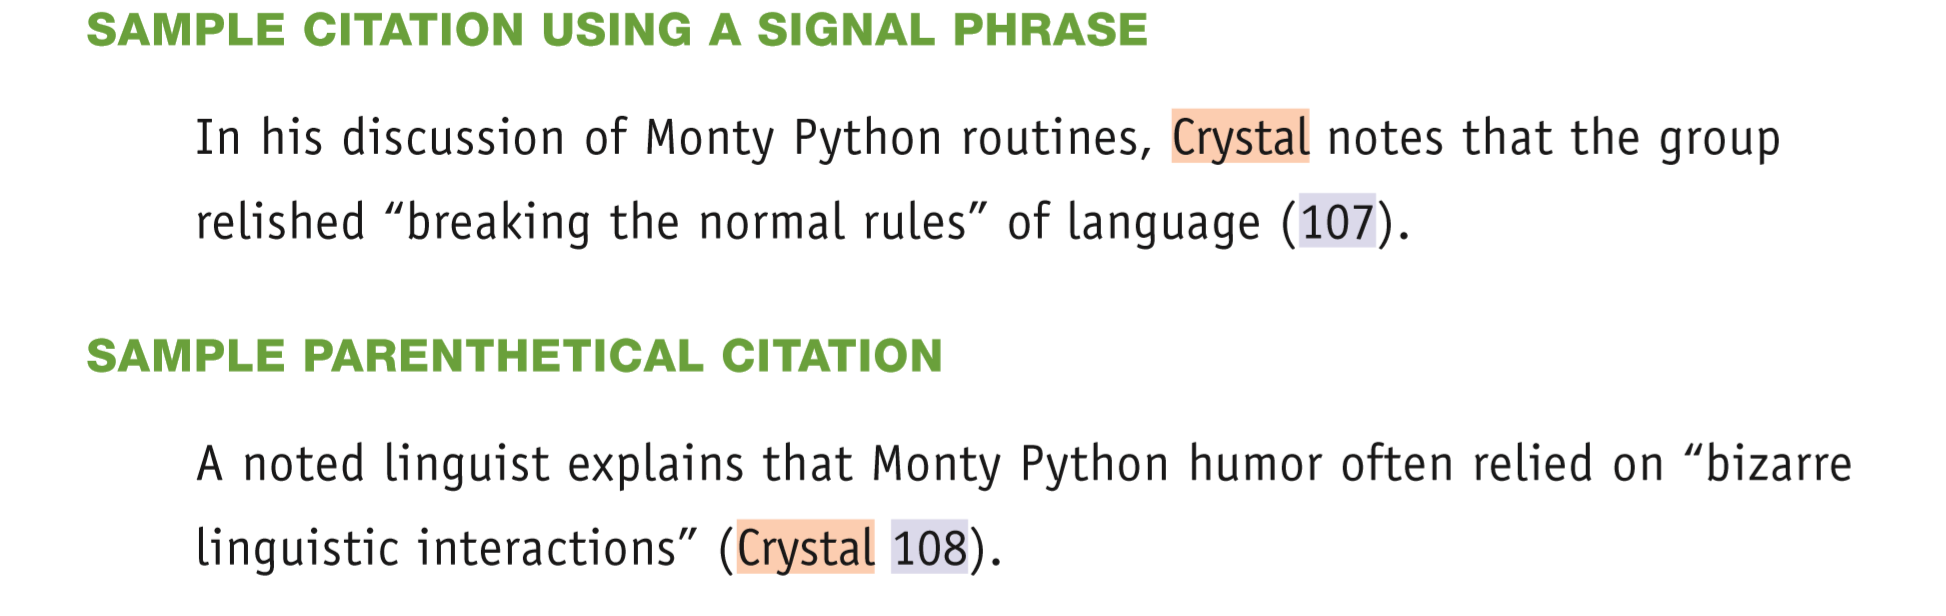
\includegraphics[width=12cm]{intext.png}
\end{figure}
\end{frame}
%------------------------------------------------
\begin{frame}
\frametitle{In-text Citation}
Cases when the author is not a single person/indirect speech/time-based video. Read pp. 465-469.
\begin{figure}[!htbp]
\center
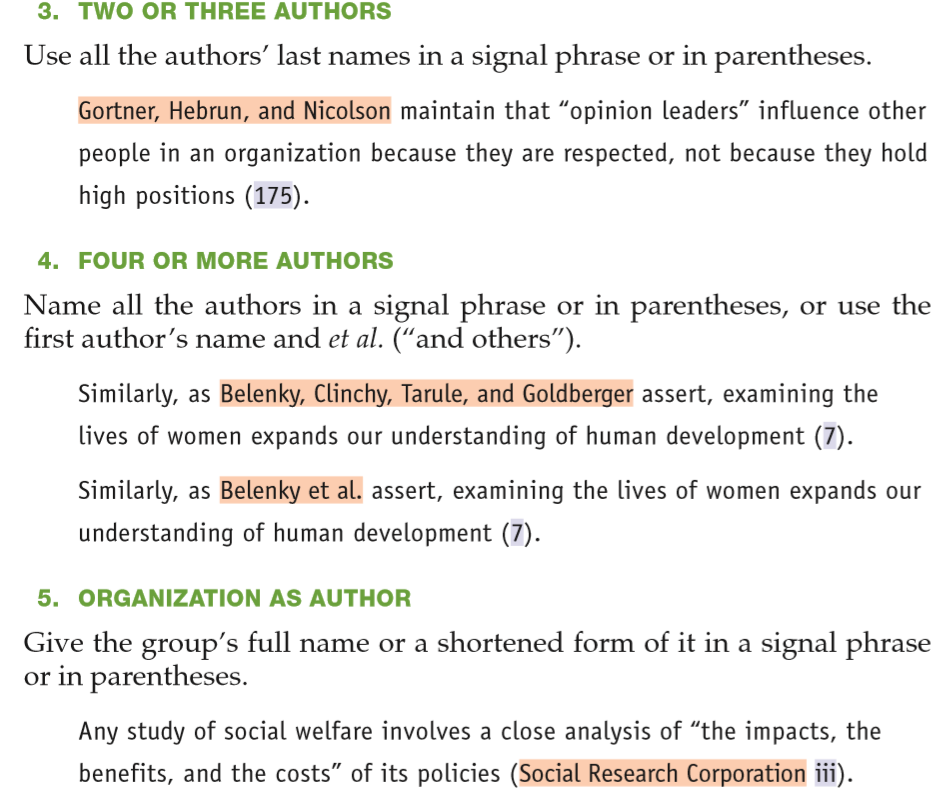
\includegraphics[width=8cm]{author1.png}
\end{figure}
\end{frame}
%------------------------------------------------
\begin{frame}
\frametitle{In-text Citation}
Cases when the author is not a single person/indirect speech/time-based video. Read pp. 465-469.
\begin{figure}[!htbp]
\center
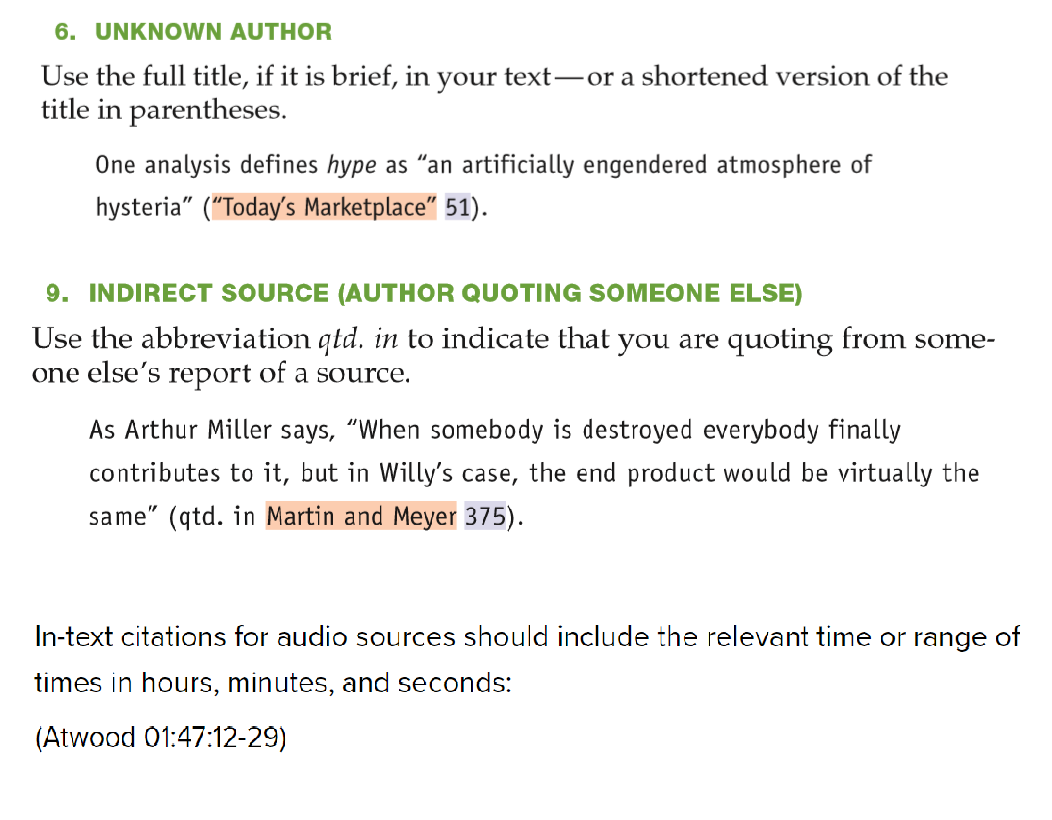
\includegraphics[width=8cm]{author2.png}
\end{figure}
\end{frame}
%------------------------------------------------
\begin{frame}
\frametitle{Works Cited List}
The list of works cited is arranged \textbf{alphabetically}. Rules for author listing is as follows.
\begin{figure}[!htbp]
\center
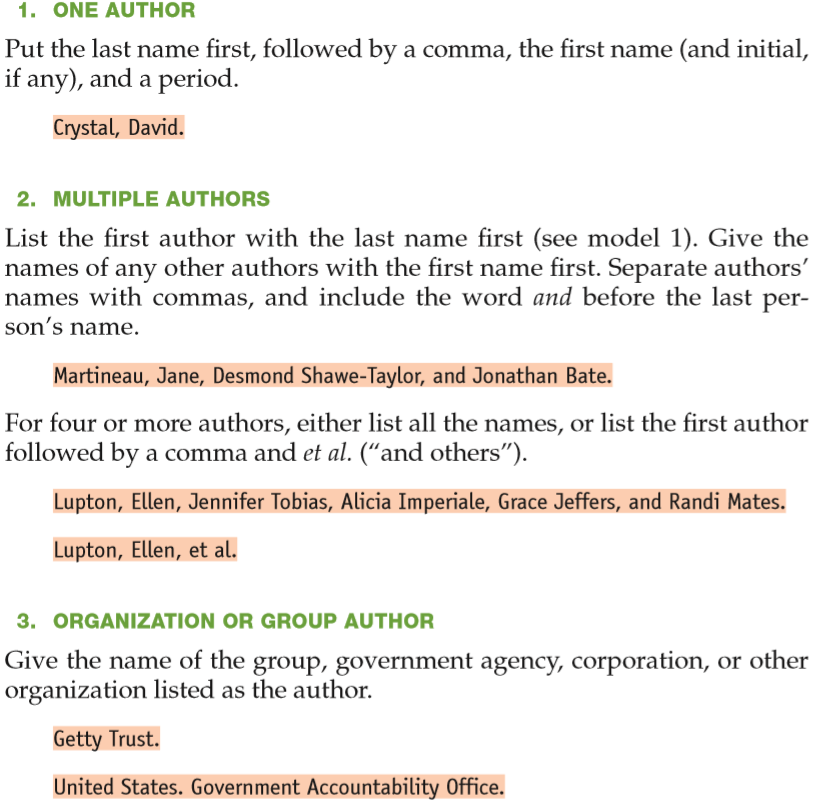
\includegraphics[width=6cm]{author3.png}
\end{figure}
\end{frame}
%------------------------------------------------
\begin{frame}
\frametitle{Works Cited List}
\begin{figure}[!htbp]
\center
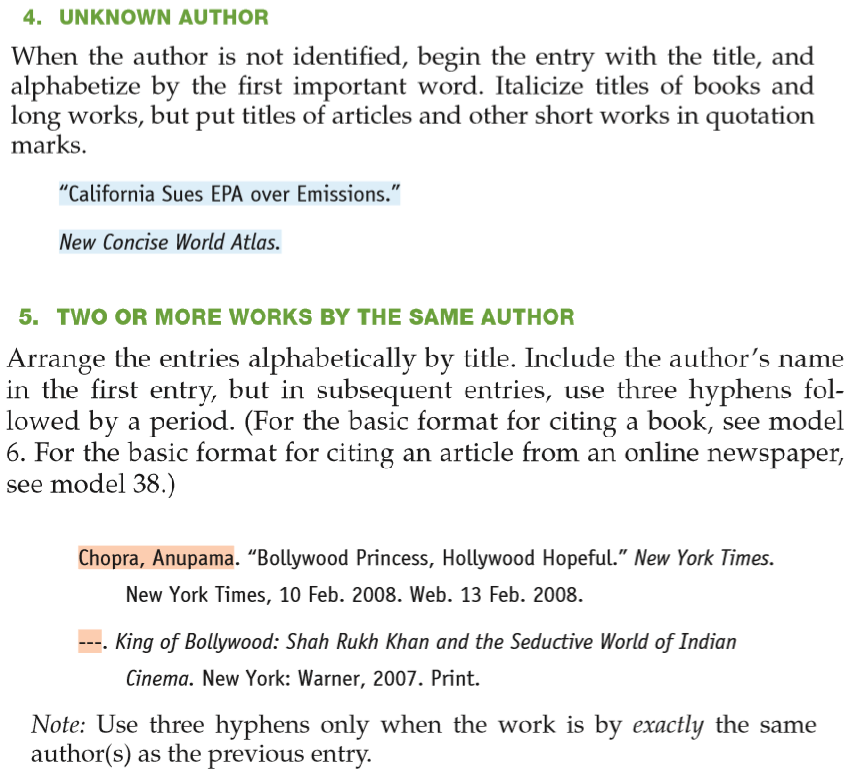
\includegraphics[width=8cm]{author4.png}
\end{figure}
\end{frame}
%------------------------------------------------
\begin{frame}
\frametitle{Works Cited List}
Format for printed books.
\begin{figure}[!htbp]
\center
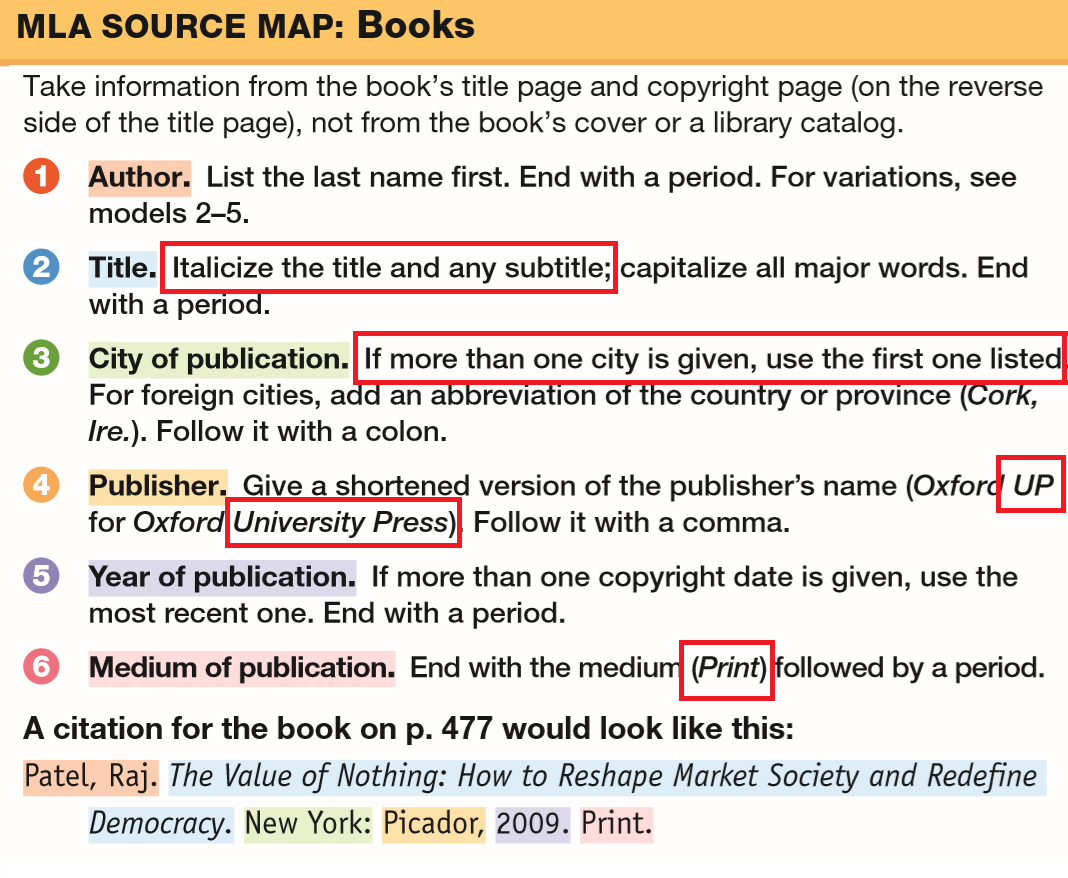
\includegraphics[width=8cm]{book.png}
\end{figure}
\end{frame}
%------------------------------------------------
\begin{frame}
\frametitle{Works Cited List}
Format for websites.
\begin{figure}[!htbp]
\center
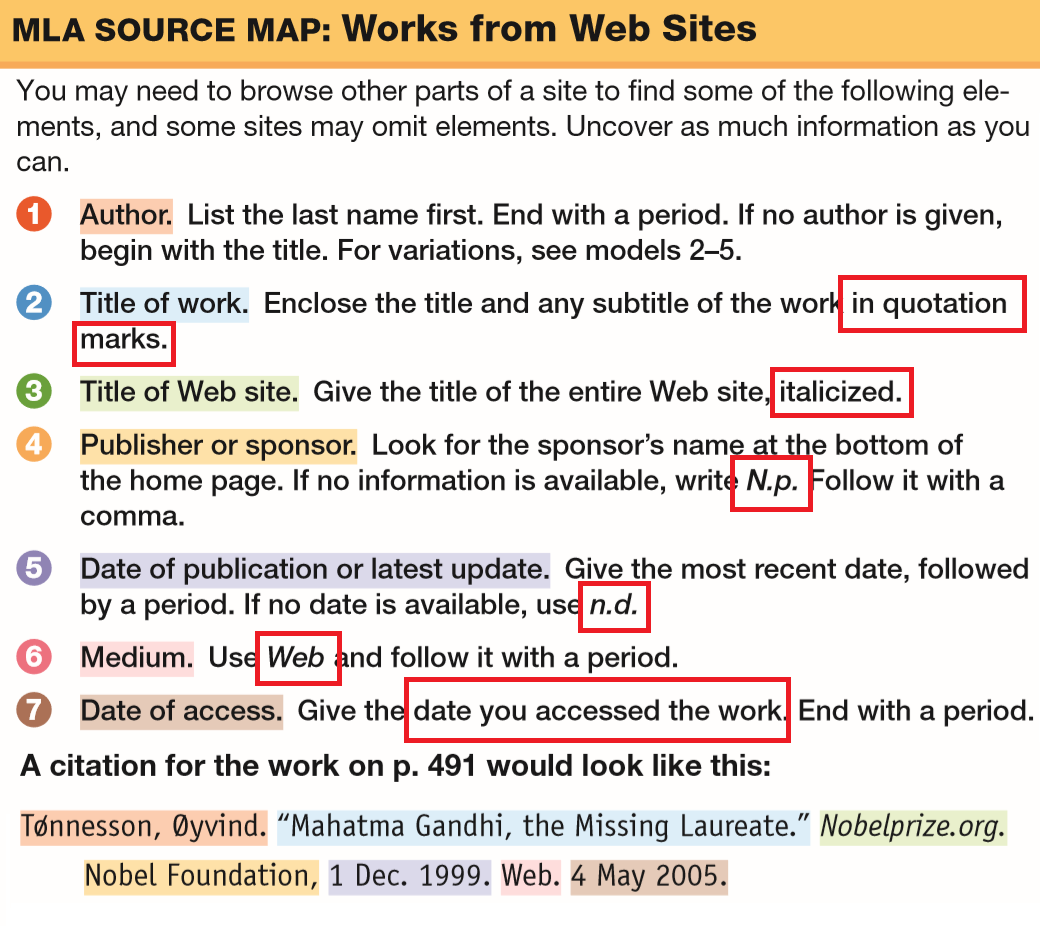
\includegraphics[width=8cm]{web.png}
\end{figure}
\end{frame}
%------------------------------------------------
\begin{frame}
\frametitle{Works Cited List}
Format for databases.
\begin{figure}[!htbp]
\center
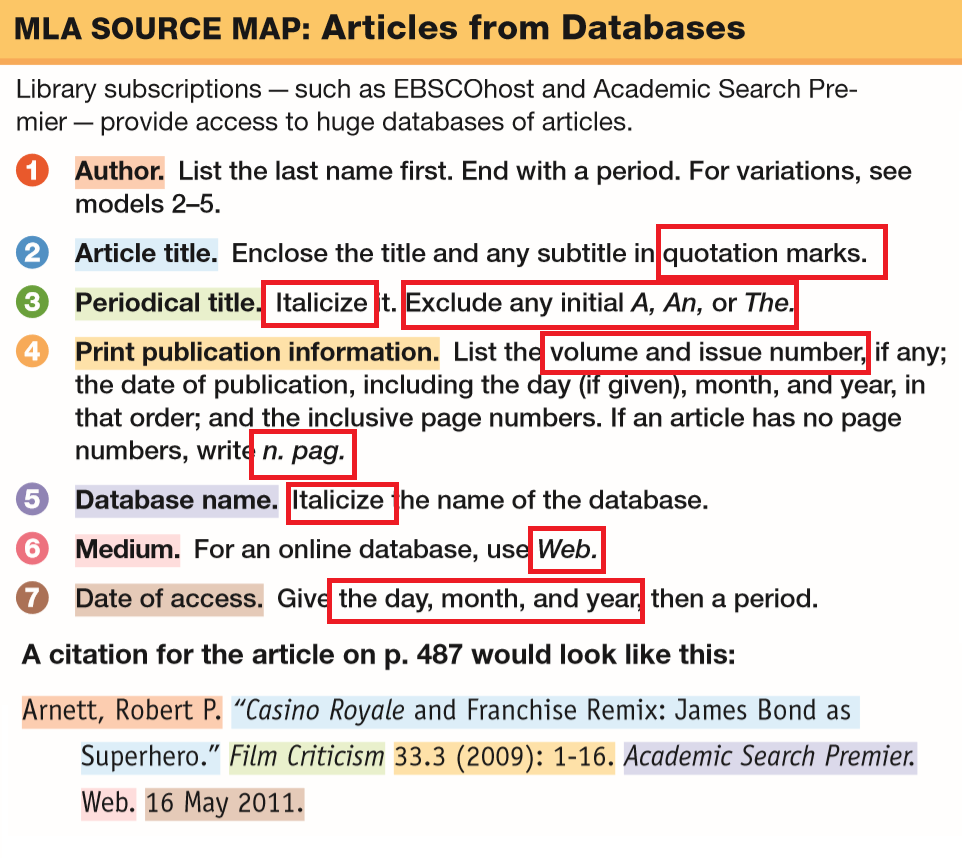
\includegraphics[width=8cm]{database.png}
\end{figure}
\end{frame}
%------------------------------------------------
\begin{frame}
\frametitle{Works Cited List}
Format for TV series episodes.
\begin{figure}[!htbp]
\center
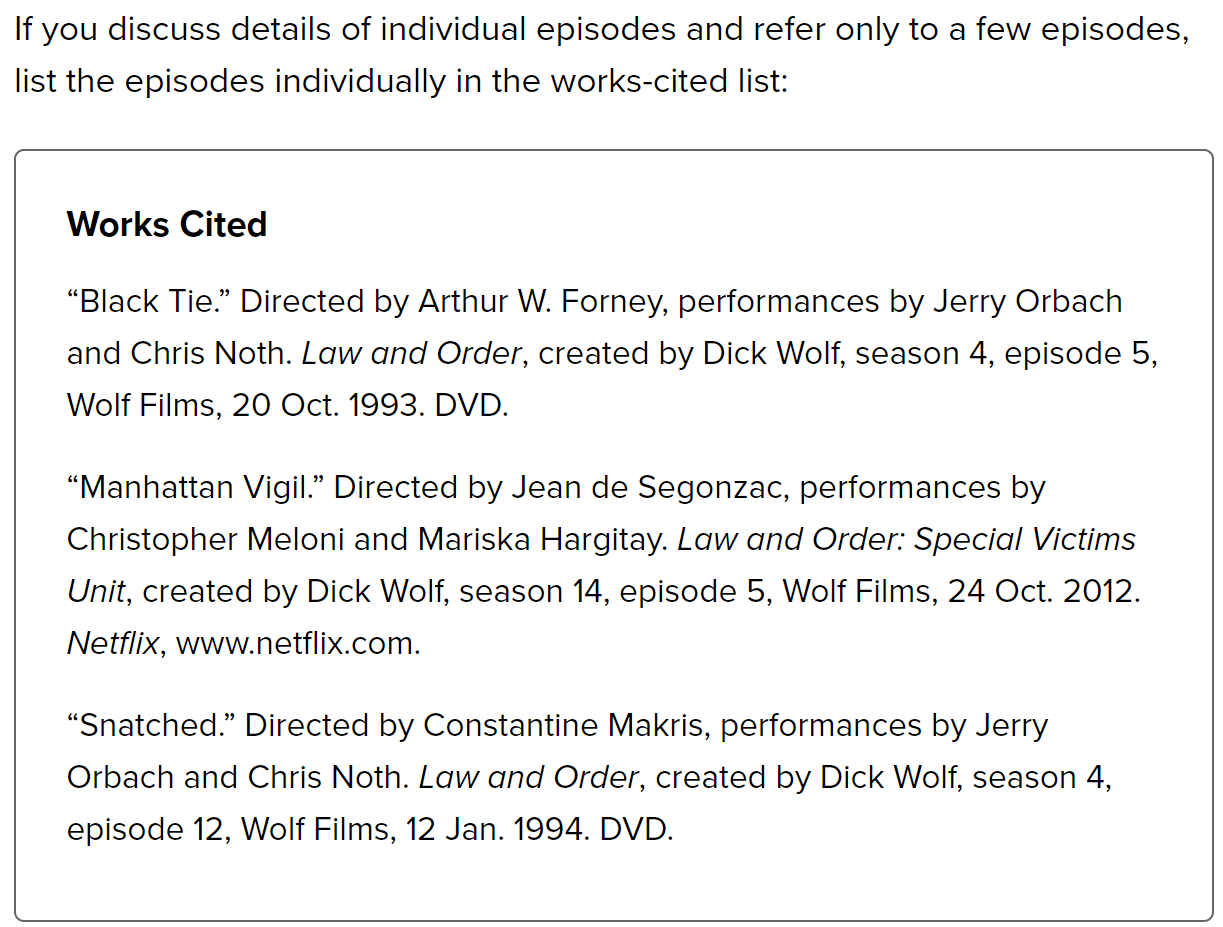
\includegraphics[width=8cm]{episode.png}
\end{figure}
\end{frame}
\section{Reading Materials}
%------------------------------------------------
\begin{frame}
\frametitle{Reading}
All the reading materials published so far may be present in your midterm. If you have read them, you should be OK with the questions.
\begin{figure}[!htbp]
\center
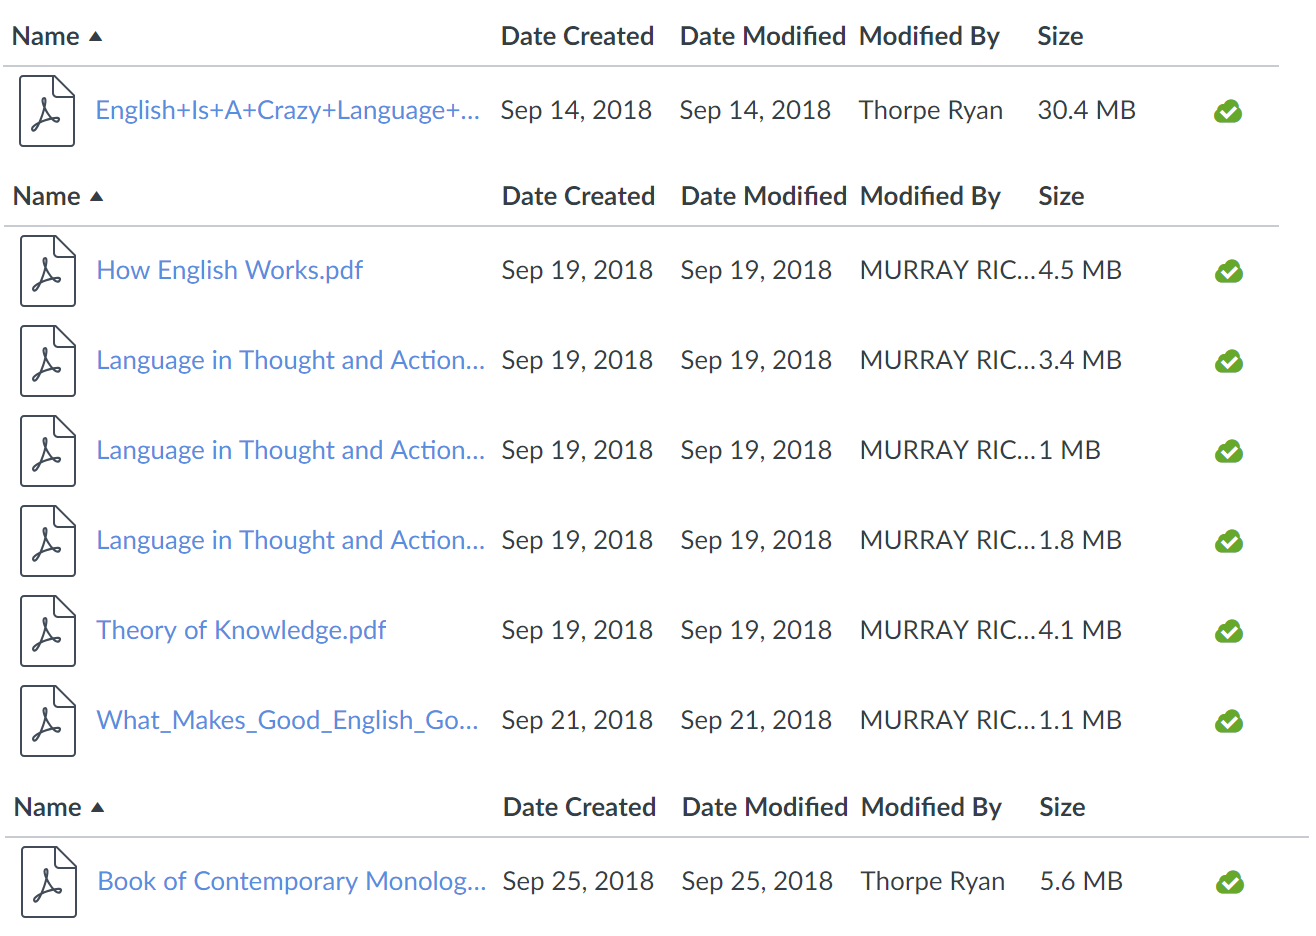
\includegraphics[width=8cm]{reading.png}
\end{figure}
\end{frame}
%------------------------------------------------
\section{References}
\begin{frame}
\frametitle{About the Midterm}
\begin{itemize}
\item Exam time: \textbf{2018/11/11 Sun. 12:10-13:50}.
\item Exam room: \textbf{Dong Zhong Yuan 2-101}. Arrive early.
\item \textbf{No cheating paper or dictionary of any kind are allowed}. For detailed rules, refer to SJTU examination rules posed on Canvas.
\item 100 min should be enough for those who are familiar with the contents, so you don't need to rush through the test.
\item When you cannot give the exact answer, give explanations at least. This will earn you partial credits.
\item Word banks will be provided so no worrying about difficult spellings.
\end{itemize}
\end{frame}
%------------------------------------------------
\begin{frame}
\frametitle{References}
\footnotesize{
\begin{thebibliography}{99} % Beamer does not support BibTeX so references must be inserted manually as below
\bibitem[Lunsford, 2013]{p1} Andrea A. Lunsford  (2013)
\newblock The Everyday Writer (5th ed)
\newblock \emph{Bedford/St. Martin's}, Boston.

\end{thebibliography}
}
\end{frame}
%------------------------------------------------
\begin{frame}
\Huge{\centerline{Good Luck :)}}
\end{frame}
%----------------------------------------------------------------------------------------
\end{document}
